\documentclass[10pt,twocolumn,a4paper]{article}

% -----------------------------------------------------------------------------
% Algorithmica inspired A4 two-column manuscript.
% The layout follows the supplied publishing template: A4 page, 0.75 inch top,
% 1.18 inch bottom, 0.51 inch side margins, and approximately 0.25 inch column gap.
% -----------------------------------------------------------------------------
\usepackage[a4paper,top=0.75in,bottom=1.18in,left=0.51in,right=0.51in,columnsep=0.25in]{geometry}
\usepackage[T1]{fontenc}
\usepackage[utf8]{inputenc}
\usepackage{amsmath,amssymb,mathtools}
\usepackage{amsthm}
\usepackage{newtxtext,newtxmath}
\usepackage{microtype}
\usepackage{xspace}
\usepackage{bm}
\usepackage{booktabs,multirow,array,tabularx}
\usepackage{graphicx}
\usepackage{caption}
\usepackage{subcaption}
\usepackage{algorithm}
\usepackage{algpseudocode}
\usepackage{enumitem}
\usepackage{xcolor}
\usepackage{tikz}
\usetikzlibrary{arrows.meta,positioning,fit,calc,shapes.geometric,shapes.multipart,backgrounds,matrix,decorations.pathreplacing}
\usepackage{pgfplots}
\pgfplotsset{compat=1.18}
\usepackage{hyperref}
\usepackage{url}
\usepackage{cleveref}
\usepackage{fancyhdr}
\usepackage{balance}
\usepackage{stfloats}
\usepackage{cuted}

\definecolor{algblue}{RGB}{30,80,145}
\definecolor{alggreen}{RGB}{24,126,96}
\definecolor{algorange}{RGB}{190,102,26}
\definecolor{algred}{RGB}{165,47,47}
\definecolor{algray}{RGB}{241,243,246}
\definecolor{algpurple}{RGB}{93,66,145}

\hypersetup{
  colorlinks=true,
  linkcolor=algblue,
  citecolor=algblue,
  urlcolor=algblue,
  pdfauthor={Panashe Chiurunge},
  pdftitle={Coherent Multi-Teacher Knowledge Distillation through Multi-Agent Reinforcement Learning}
}

\pagestyle{fancy}
\fancyhf{}
\fancyhead[L]{\footnotesize\itshape Algorithmica: International Journal of Computational Sciences}
\fancyhead[R]{\footnotesize Volume 1, Issue 1, 2026, ISSN Online: 3106-1435}
\fancyfoot[L]{\footnotesize\itshape http://africau.edu/}
\fancyfoot[R]{\footnotesize\thepage}
\renewcommand{\headrulewidth}{0pt}
\renewcommand{\footrulewidth}{0pt}
\setlength{\headheight}{14pt}

\setlength{\parindent}{1em}
\setlength{\parskip}{0pt}
\setlist[itemize]{leftmargin=*,topsep=2pt,itemsep=1pt,parsep=0pt}
\setlist[enumerate]{leftmargin=*,topsep=2pt,itemsep=1pt,parsep=0pt}
\captionsetup{font=footnotesize,labelfont=bf}
\captionsetup[table]{position=top}
\renewcommand{\figurename}{Fig.}
\renewcommand{\tablename}{TABLE}

\newtheorem{definition}{Definition}
\newtheorem{assumption}{Assumption}
\newtheorem{theorem}{Theorem}
\newtheorem{lemma}{Lemma}
\newtheorem{proposition}{Proposition}
\newtheorem{corollary}{Corollary}
\newtheorem{remark}{Remark}
\newtheorem{hypothesis}{Hypothesis}

\newcommand{\R}{\mathbb{R}}
\newcommand{\E}{\mathbb{E}}
\newcommand{\Pp}{\mathbb{P}}
\newcommand{\KL}{D_{\mathrm{KL}}}
\newcommand{\JS}{D_{\mathrm{JS}}}
\newcommand{\TV}{D_{\mathrm{TV}}}
\newcommand{\cX}{\mathcal{X}}
\newcommand{\cR}{\mathcal{R}}
\newcommand{\cT}{\mathcal{T}}
\newcommand{\cS}{\mathcal{S}}
\newcommand{\cD}{\mathcal{D}}
\newcommand{\cL}{\mathcal{L}}
\newcommand{\cG}{\mathcal{G}}
\newcommand{\cA}{\mathcal{A}}
\newcommand{\cO}{\mathcal{O}}
\newcommand{\cM}{\mathcal{M}}
\newcommand{\cK}{\mathcal{K}}
\newcommand{\cV}{\mathcal{V}}
\newcommand{\cI}{\mathcal{I}}
\newcommand{\cJ}{\mathcal{J}}
\newcommand{\simplex}{\Delta}
\newcommand{\ind}{\mathbf{1}}
\newcommand{\diag}{\operatorname{Diag}}
\newcommand{\softmax}{\operatorname{softmax}}
\newcommand{\sparsemax}{\operatorname{sparsemax}}
\newcommand{\Tr}{\operatorname{Tr}}
\newcommand{\rank}{\operatorname{rank}}
\newcommand{\relu}{\operatorname{ReLU}}
\newcommand{\clip}{\operatorname{clip}}
\newcommand{\CoMTKD}{\textsc{CoMTKD-MARL}\xspace}

\makeatletter
\newcommand{\fullwidthtitle}{%
\twocolumn[
\begin{@twocolumnfalse}
\begin{center}
{\fontsize{24}{28}\selectfont\rmfamily Coherent Multi-Teacher Knowledge Distillation through Multi-Agent Reinforcement Learning:\\[2pt]
A Formal Theory of Knowledge Aggregation, Synchronization, and Optimal Teacher Cardinality\par}
\vspace{0.65em}
{\fontsize{14}{17}\selectfont Panashe Chiurunge\par}
\vspace{0.25em}
{\fontsize{10}{12}\selectfont Deep Analytics (Pvt) Ltd, Harare, Zimbabwe\par}
{\fontsize{10}{12}\selectfont panashe@deepanalytics.ml\par}
\end{center}
\vspace{0.6em}
\noindent\textbf{Abstract}: Multi-teacher knowledge distillation can expose a compact student to complementary predictive, representational, and relational knowledge. Existing methods mainly optimize teacher weights from confidence or teacher-student discrepancy, while reinforcement learning based methods typically place one decision agent above the teacher pool. This formulation does not explicitly coordinate the teachers, synchronize the knowledge being transferred, quantify redundancy and conflict, or determine when an additional teacher no longer improves learning. This paper develops Coherent Multi-Teacher Knowledge Distillation with Multi-Agent Reinforcement Learning, a framework in which each teacher is represented by a cooperative knowledge agent. The agents select participation, teaching strength, temperature, and knowledge channels from local observations, while a centralized coherence critic and a synchronization operator coordinate the joint teaching policy during training. The student remains independent at inference. The framework aggregates calibrated logits, projected features, relational structure, uncertainty, and marginal novelty, and it penalizes epistemic disagreement, duplicated information, unstable weighting, communication cost, and student-capacity mismatch. Three formal results organize the theory. The Multi-Teacher Advantage Theorem gives sufficient covariance and transfer conditions under which a coordinated teacher coalition has lower expected risk than every admissible single teacher. The Knowledge Coherence Theorem proves geometric contraction of disagreement under a connected synchronization graph and gives a nonzero robustness floor under bounded communication perturbations. The Teacher Saturation Theorem combines conditional mutual information, a bounded student information channel, and increasing coordination cost to establish a finite optimal teacher cardinality and an operational stopping rule. A complete bilevel learning objective, counterfactual credit assignment mechanism, cardinality controller, algorithms, complexity analysis, and reproducible experimental protocol are provided. The resulting theory explains both the advantage of diverse teachers and the saturation or deterioration that occurs when redundant, conflicting, or undistillable teachers are added.\par
\vspace{0.5em}
\noindent\textbf{Keywords}: coherence; knowledge aggregation; knowledge distillation; multi-agent reinforcement learning; multi-teacher learning; synchronization; teacher cardinality; teacher selection.\par
\vspace{1.1em}
\end{@twocolumnfalse}
]
}
\makeatother

\begin{document}
\fullwidthtitle

\section{Introduction}
\label{sec:intro}

Knowledge distillation transfers information from a high-capacity teacher to a smaller student by combining ground-truth supervision with softened teacher targets or intermediate representations \cite{hinton2015,romero2015}. A single teacher can regularize the student and reveal class relationships that are absent from one-hot labels, but it can also transmit its own bias, calibration error, blind spots, and representations that the student cannot absorb. The capacity gap is important. A teacher with higher standalone accuracy does not necessarily produce a better student, and some teacher classes or features may be effectively undistillable \cite{cho2019,zhu2022,stanton2021}.

Multi-teacher knowledge distillation attempts to address these limitations by combining heterogeneous teachers. Diversity can reduce correlated error, broaden class coverage, and expose complementary invariances. It can also create a harder optimization problem. Equal averaging ignores teacher quality and disagreement. Static confidence rules can overvalue a confidently wrong teacher. Sample-wise weighting can improve relevance, but independent weights do not guarantee that the resulting teaching signals are mutually compatible. Gradient conflict, repeated information, stale signals, and incompatible feature spaces can make the student chase a moving or internally inconsistent target \cite{du2020,yang2025}.

Reinforcement learning provides a natural mechanism for sequential teacher selection because the value of a teacher depends on the current student state, the sample, the active teacher coalition, and the delayed effect on validation performance. The MTKD-RL framework uses teacher performance and teacher-student gaps as the state of an agent that outputs teacher weights \cite{yang2025}. Its reported teacher-count ablation improves with more teachers and then saturates at four teachers in the evaluated setting. That observation motivates a more general question. Why should saturation occur, and can a learning system identify the useful cardinality rather than fixing it in advance?

The problem becomes a cooperative multi-agent learning problem when each teacher has a separate policy that decides what, when, and how strongly to teach. This interpretation introduces two difficulties. First, the environment observed by one teacher agent changes as the student and the other agents update. Second, separately rational actions can produce an incoherent joint target. Centralized training with decentralized execution, counterfactual credit assignment, and value factorization provide relevant tools for coordination \cite{lowe2017,foerster2018,rashid2018,yu2022}. Distributed systems theory also warns that exact global coherence cannot generally coexist with bounded memory, lossy communication, non-stationarity, and full decentralization \cite{halpern1990,chiurunge2026}. The proposed method therefore makes an explicit architectural choice. It uses a centralized coherence critic and synchronization oracle during training, then deploys only the student.

\subsection{Central Research Question}

\begin{quote}
\itshape Under what mathematical and operational conditions does a coordinated set of teachers transfer more useful knowledge than the best single teacher, how can multi-agent reinforcement learning aggregate and synchronize that knowledge, and at what point does adding teachers cease to improve the student?
\end{quote}

\subsection{Central Thesis}

The central thesis is that multiple teachers improve knowledge acquisition when four conditions hold. Their errors are not perfectly correlated, their knowledge is complementary, their signals are learnable by the student, and their joint supervision remains coherent. Additional teachers have diminishing value because conditional novelty decreases while redundancy, conflict, communication, optimization, and student-capacity costs increase. Consequently, the optimal teacher count is a learned property of the teacher pool, student, task, and training stage, rather than a fixed hyperparameter.

\subsection{Contributions}

This paper makes the following contributions.

\begin{enumerate}
    \item It formulates multi-teacher distillation as a cooperative partially observable Markov game in which every teacher is represented by an adaptive knowledge agent. Each agent controls participation, weight, temperature, and knowledge channels.
    \item It introduces a synchronization layer that maps heterogeneous teacher outputs into a shared knowledge space, performs graph-based consensus, and exposes a measurable coherence index to the centralized critic.
    \item It defines a complete bilevel objective that combines supervised learning, logit, feature, and relational distillation with cooperative reward, difference rewards, coherence penalties, redundancy control, policy stability, and cardinality cost.
    \item It proves a Multi-Teacher Advantage Theorem. The theorem connects the benefit of a teacher coalition to the second-moment matrix of teacher errors and gives a sufficient condition that includes student transfer error.
    \item It proves a Knowledge Coherence Theorem. The theorem gives geometric contraction under ideal synchronization and a bounded disagreement floor under perturbed or lossy communication.
    \item It proves a Teacher Saturation Theorem. The theorem combines conditional mutual information, student information capacity, and increasing coordination cost to establish a finite optimal teacher cardinality and a stopping criterion.
    \item It provides training, synchronization, and teacher-cardinality algorithms, together with a falsifiable experimental protocol that does not assume the proposed theorems will hold outside their stated conditions.
\end{enumerate}

\section{Related Work}
\label{sec:related}

\subsection{Single-Teacher Knowledge Distillation}

Classical knowledge distillation minimizes a mixture of supervised loss and divergence between student and teacher predictive distributions \cite{hinton2015}. Feature-based methods align intermediate representations, while relational methods transfer pairwise or structural information. FitNets use intermediate hints to train a thinner student \cite{romero2015}. Subsequent research has shown that teacher quality alone is insufficient. The student-teacher capacity gap, optimization dynamics, class-specific incompatibility, and data used for transfer affect whether the student can benefit \cite{cho2019,stanton2021,zhu2022,park2021}. These findings motivate explicit compatibility terms in the state of each teacher agent.

\subsection{Multi-Teacher Distillation}

A simple multi-teacher objective averages the losses induced by all teachers. This can reduce variance when teacher errors are weakly correlated, but it can also create destructive gradient interference. Adaptive ensemble knowledge distillation treats teacher losses as a multi-objective optimization problem and uses gradient geometry to account for disagreement \cite{du2020}. Other approaches estimate confidence, entropy, teacher-student similarity, or meta-learned importance. MTKD-RL combines teacher performance and teacher-student gaps in a reinforcement learning state and learns continuous teacher weights from student feedback \cite{yang2025}. The present work differs in three respects. It uses one cooperative actor per teacher, it coordinates their actions through a centralized critic and synchronization layer, and it treats teacher cardinality as a decision variable with a formal saturation criterion.

\subsection{Teacher Selection and Student Compatibility}

Teacher selection can be viewed as a data-dependent model selection problem. Recent work uses gradient coverage and variance to predict whether a particular teacher will be useful for a student \cite{panigrahi2026}. Student-friendly teacher training and class filtering address incompatible representations and undistillable classes \cite{park2021,zhu2022}. The proposed method incorporates compatibility, gradient alignment, and marginal novelty directly into each teacher observation, then lets the joint policy trade them against cost and coherence.

\subsection{Multi-Agent Reinforcement Learning}

Independent learners face non-stationarity because every agent changes the environment observed by the others. MADDPG addresses this problem with centralized critics and decentralized actors \cite{lowe2017}. COMA uses a centralized critic and counterfactual baseline for credit assignment \cite{foerster2018}. QMIX factorizes a joint action-value under a monotonicity constraint \cite{rashid2018}. MAPPO demonstrates that carefully implemented proximal policy optimization is a strong cooperative multi-agent baseline \cite{yu2022}. \CoMTKD adopts centralized training because all teacher logits, features, student gradients, and validation feedback are available during distillation. There is no requirement to retain the teacher agents after deployment.

\subsection{Synchronization, Epistemic Divergence, and Bounded Information}

Consensus algorithms converge when the communication graph is sufficiently connected and the mixing operator has a spectral gap \cite{olfati2007,boyd2006}. Exact common knowledge is generally unattainable over unreliable asynchronous channels \cite{halpern1990}. A broader failure theory links epistemic divergence, non-stationary learning, bounded communication, and memory decay, and proposes coherence indicators and an oracle-based mitigation \cite{chiurunge2026}. The present paper applies that insight to distillation. The training-time synchronization oracle is an explicit relaxation of full decentralization, used to make teacher messages comparable and coherent.

\subsection{Submodularity and Information Saturation}

If teacher signals are conditionally independent given the target, the information obtained from a set of teachers often exhibits diminishing returns. Submodular optimization provides approximation results for selecting informative subsets under cost constraints \cite{nemhauser1978,krause2014}. Information bottleneck theory provides a complementary ceiling. A bounded student representation cannot preserve arbitrary information from an expanding teacher coalition \cite{tishby1999,cover2006}. These ideas support the Teacher Saturation Theorem in \cref{sec:theory}.

\section{Problem Formulation}
\label{sec:problem}

\subsection{Data, Teachers, and Student}

Let \(\cD\) be a distribution over input-label pairs \((X,Y)\in\cX\times\{1,\ldots,C\}\). A pool of \(M\) pretrained teachers is
\begin{equation}
\cT=\{T_m\}_{m=1}^{M}.
\end{equation}
Teacher \(T_m\) produces logits \(z_m(x)\in\R^C\), predictive probabilities at temperature \(\tau_m>0\),
\begin{equation}
 p_m^{(\tau_m)}(y\mid x)
 =\frac{\exp(z_{m,y}(x)/\tau_m)}{\sum_{c=1}^{C}\exp(z_{m,c}(x)/\tau_m)},
\label{eq:teacherprob}
\end{equation}
and one or more intermediate features \(h_m^{(\ell)}(x)\). The student \(S_\theta\) produces \(q_\theta^{(\tau)}(y\mid x)\) and features \(h_S^{(\ell)}(x)\).

Teacher architectures can be heterogeneous. A learned adapter \(A_m^{(\ell)}\) maps each selected teacher feature into a common \(d_\ell\)-dimensional space,
\begin{equation}
 k_m^{(\ell)}(x)=A_m^{(\ell)}h_m^{(\ell)}(x)\in\R^{d_\ell}.
\label{eq:adapter}
\end{equation}
The complete teacher knowledge packet is
\begin{equation}
 \kappa_m(x)=\left[p_m^{(\tau_m)}(x),\{k_m^{(\ell)}(x)\}_{\ell\in\cL},r_m(x),u_m(x)\right],
\label{eq:packet}
\end{equation}
where \(r_m(x)\) contains relational descriptors such as normalized Gram matrices, and \(u_m(x)\) contains uncertainty and calibration estimates.

\subsection{Teacher Agents}

Each teacher \(T_m\) is paired with an actor \(\pi_{\omega_m}\). At decision epoch \(t\), actor \(m\) observes
\begin{align}
 o_{m,t}=[&\ell_{m,t}^{\mathrm{sup}},\ H(p_{m,t}),\ \mathrm{ECE}_{m,t},\
 \KL(p_{m,t}\Vert q_{\theta_t}),\nonumber\\
 &d_f(k_{m,t},k_{S,t}),\ a_{m,t}^{\mathrm{grad}},\ n_{m,t},\rho_{m,t},\xi_{m,t},c_{m,t}],
\label{eq:observation}
\end{align}
where \(H\) is entropy, \(d_f\) is feature discrepancy, \(a_{m,t}^{\mathrm{grad}}\) is gradient alignment with the supervised gradient, \(n_{m,t}\) is novelty relative to active peers, \(\rho_{m,t}\) is redundancy, \(\xi_{m,t}\) is conflict, and \(c_{m,t}\) is cost or staleness.

The action is
\begin{equation}
 a_{m,t}=(g_{m,t},\alpha_{m,t},\tau_{m,t},\bm\beta_{m,t}),
\label{eq:action}
\end{equation}
where \(g_{m,t}\in[0,1]\) is a differentiable participation gate, \(\alpha_{m,t}\in\R\) is an unnormalized importance score, \(\tau_{m,t}\) is the selected temperature, and \(\bm\beta_{m,t}\in\simplex^{K-1}\) allocates mass across \(K\) teaching channels, for example logits, features, relations, and uncertainty.

The normalized teacher weights are
\begin{equation}
 w_{m,t}=\frac{g_{m,t}\exp(\alpha_{m,t})}{\sum_{j=1}^{M}g_{j,t}\exp(\alpha_{j,t})+\varepsilon},
\qquad \bm w_t\in\simplex^{M-1}.
\label{eq:weights}
\end{equation}
A hard active set can be sampled with a binary Concrete estimator during training and thresholded during evaluation \cite{jang2017}.

\subsection{Cooperative Markov Game}

The distillation process is represented as a cooperative partially observable Markov game
\begin{equation}
\cM=\langle \cA,\cS,\{\cO_m\}_{m=1}^{M},\{\cA_m\}_{m=1}^{M},P,R,\gamma\rangle,
\label{eq:markovgame}
\end{equation}
where the agents are the teacher actors, the global state contains student parameters, teacher statistics, validation history, and communication state, and all agents share a team reward. A transition consists of one or more student optimization steps under the joint teaching action. This makes the environment non-stationary from each local actor's perspective, but stationary for a centralized critic conditioned on the joint state and joint action.

\subsection{Design Assumptions}

\begin{assumption}[Comparable knowledge space]
For every selected feature level, each teacher has an adapter into a shared finite-dimensional space. Adapter error is bounded in expectation by \(\epsilon_A\).
\end{assumption}

\begin{assumption}[Bounded teacher loss and messages]
Teacher probabilities lie in the interior of the simplex, feature packets have bounded norm, and per-sample distillation losses are bounded by \(L_{\max}\).
\end{assumption}

\begin{assumption}[Training-time coordination]
During centralized training, the critic can observe the joint teacher state, joint action, student state, and a validation reward. Communication perturbations are either absent or bounded.
\end{assumption}

\begin{assumption}[Student transfer budget]
For any teacher coalition, the optimization and approximation error of the student relative to the synchronized target is finite and measurable. The student's effective distilled representation has bounded information capacity \(B_S\).
\end{assumption}

\begin{assumption}[Diminishing informational novelty]
Along the cardinality-controller selection sequence, conditional teacher information gains are nonincreasing. This condition holds, for example, for conditionally independent sensor-style teacher observations under standard entropy objectives.
\end{assumption}

\section{The CoMTKD-MARL Architecture}
\label{sec:architecture}

\begin{figure*}[t]
\centering
\resizebox{0.98\textwidth}{!}{%
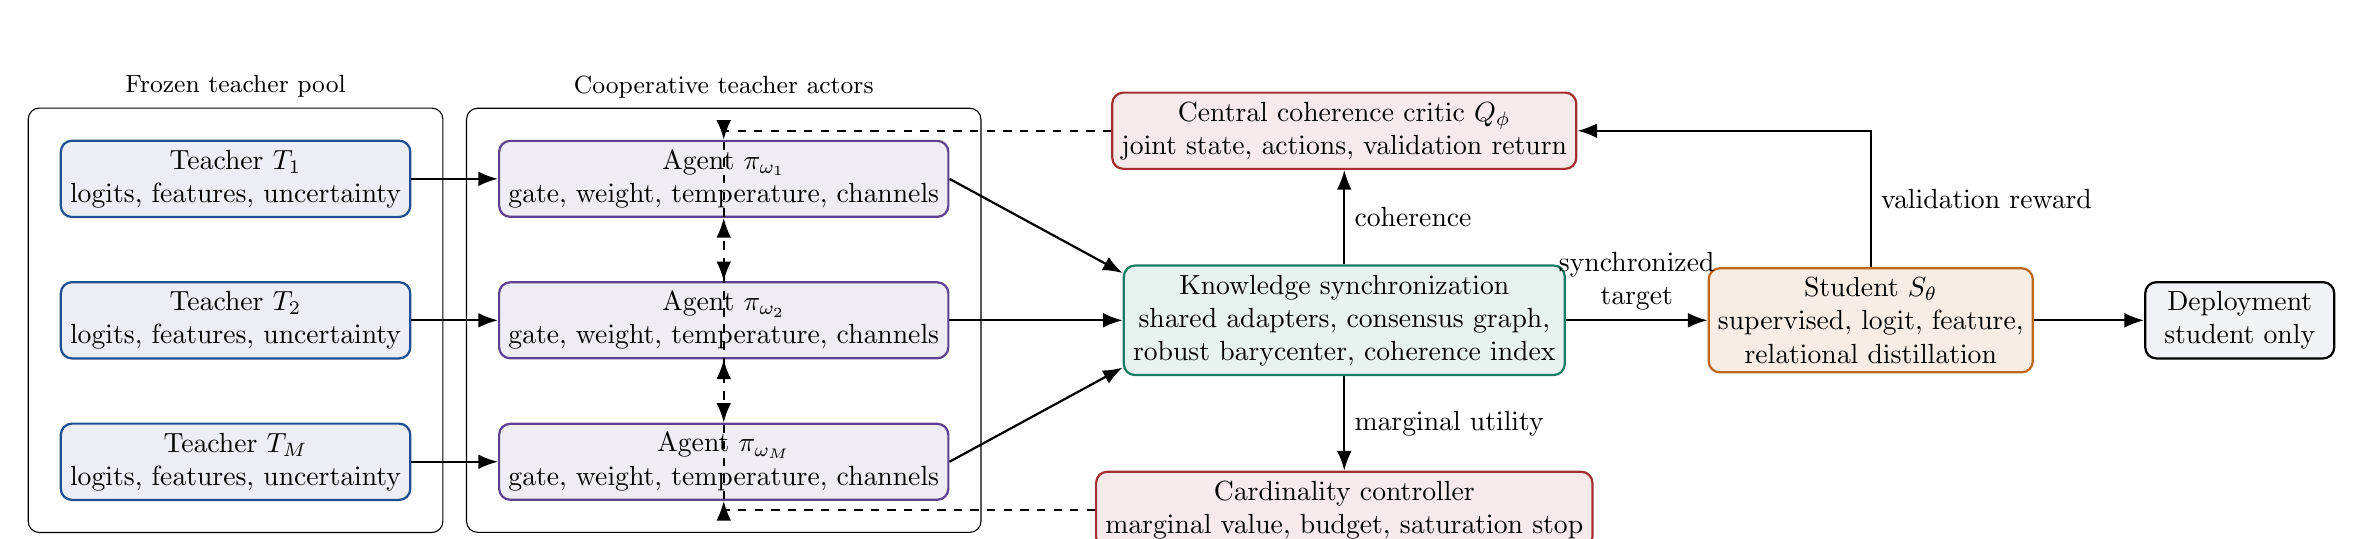
\begin{tikzpicture}[
  node distance=8mm and 11mm,
  box/.style={draw,rounded corners,thick,align=center,minimum height=9mm,minimum width=24mm,fill=white},
  teacher/.style={box,fill=algblue!9,draw=algblue},
  agent/.style={box,fill=algpurple!10,draw=algpurple},
  sync/.style={box,fill=alggreen!10,draw=alggreen,minimum width=35mm},
  student/.style={box,fill=algorange!12,draw=algorange,minimum width=31mm},
  critic/.style={box,fill=algred!10,draw=algred,minimum width=32mm},
  arr/.style={-{Latex[length=2.5mm]},thick},
  darr/.style={-{Latex[length=2.5mm]},thick,dashed}
]

\node[teacher] (t1) {Teacher $T_1$\\logits, features, uncertainty};
\node[teacher,below=of t1] (t2) {Teacher $T_2$\\logits, features, uncertainty};
\node[teacher,below=of t2] (tm) {Teacher $T_M$\\logits, features, uncertainty};
\node[agent,right=of t1] (a1) {Agent $\pi_{\omega_1}$\\gate, weight, temperature, channels};
\node[agent,right=of t2] (a2) {Agent $\pi_{\omega_2}$\\gate, weight, temperature, channels};
\node[agent,right=of tm] (am) {Agent $\pi_{\omega_M}$\\gate, weight, temperature, channels};
\node[sync,right=22mm of a2] (sync) {Knowledge synchronization\\shared adapters, consensus graph,\\robust barycenter, coherence index};
\node[student,right=18mm of sync] (student) {Student $S_\theta$\\supervised, logit, feature,\\relational distillation};
\node[critic,above=12mm of sync] (critic) {Central coherence critic $Q_\phi$\\joint state, actions, validation return};
\node[critic,below=12mm of sync] (card) {Cardinality controller\\marginal value, budget, saturation stop};
\node[box,right=14mm of student,fill=algray] (deploy) {Deployment\\student only};

\draw[arr] (t1) -- (a1);
\draw[arr] (t2) -- (a2);
\draw[arr] (tm) -- (am);
\draw[arr] (a1.east) -- ([yshift=6mm]sync.west);
\draw[arr] (a2.east) -- (sync.west);
\draw[arr] (am.east) -- ([yshift=-6mm]sync.west);
\draw[arr] (sync) -- node[above,align=center]{synchronized\\target} (student);
\draw[arr] (student) -- (deploy);
\draw[darr] (critic.west) -| (a1.north);
\draw[darr] (critic.west) -| (a2.north);
\draw[darr] (critic.west) -| (am.north);
\draw[arr] (student.north) |- node[pos=0.25,right]{validation reward} (critic.east);
\draw[arr] (sync.north) -- node[right]{coherence} (critic.south);
\draw[darr] (card.west) -| (a1.south);
\draw[darr] (card.west) -| (a2.south);
\draw[darr] (card.west) -| (am.south);
\draw[arr] (sync.south) -- node[right]{marginal utility} (card.north);

\node[draw,rounded corners,fit=(t1)(tm),inner sep=4mm,label=above:{\small Frozen teacher pool}] {};
\node[draw,rounded corners,fit=(a1)(am),inner sep=4mm,label=above:{\small Cooperative teacher actors}] {};
\end{tikzpicture}}
\caption{The \CoMTKD architecture. Teacher models remain frozen by default. Each teacher actor chooses participation and teaching parameters. A synchronization module produces a coherent target, a centralized critic assigns cooperative credit, and a cardinality controller removes teachers whose marginal value is non-positive. Only the student is required at inference.}
\label{fig:architecture}
\end{figure*}

\subsection{Teacher Knowledge Encoders}

Every teacher is converted into a knowledge packet by temperature calibration, feature adaptation, and relational projection. Calibration can be performed on a held-out split before MARL training, or temperature can be part of the actor action. Feature adapters can be linear maps, small multilayer perceptrons, or dimension-preserving projection heads. To prevent the adapters from hiding teacher disagreement, they are regularized with reconstruction and orthogonality terms,
\begin{equation}
\cL_{\mathrm{adapt}}
=\sum_{m,\ell}\left\|B_m^{(\ell)}A_m^{(\ell)}h_m^{(\ell)}-h_m^{(\ell)}\right\|_2^2
+\lambda_O\left\|A_m^{(\ell)}A_m^{(\ell)\top}-I\right\|_F^2.
\label{eq:adapterloss}
\end{equation}

\subsection{Teacher Actor Network}

A teacher actor contains a local observation encoder, a recurrent state for delayed reward, and four output heads corresponding to \cref{eq:action}. Parameter sharing is optional. When teachers have heterogeneous architectures and domains, a shared backbone with learned teacher identifiers gives permutation-aware generalization without forcing identical policies. The actor does not directly alter teacher parameters. It controls how the teacher's frozen knowledge enters the student objective.

\subsection{Synchronization and Coherence Oracle}

The synchronization module receives the active packets and weights. It has three responsibilities.

\begin{enumerate}
    \item It maps heterogeneous representations into common spaces.
    \item It performs finite-round graph consensus or centralized barycentric aggregation.
    \item It computes coherence, redundancy, conflict, and marginal novelty indicators for the critic and cardinality controller.
\end{enumerate}

This module is called an oracle because it sees the active teacher coalition during training. It is not assumed to know the true label distribution. Its role is coordination, not omniscience.

\subsection{Centralized Critic and Counterfactual Credit}

The critic \(Q_\phi(s_t,\bm a_t)\) sees the global state and all teacher actions. It predicts the discounted student-improvement return. To assign credit to teacher \(m\), the framework uses a counterfactual baseline,
\begin{equation}
 A_{m,t}^{\mathrm{cf}}
 =Q_\phi(s_t,\bm a_t)
 -\E_{a'_m\sim\pi_{\omega_m}(\cdot\mid o_{m,t})}
 Q_\phi(s_t,(\bm a_{-m,t},a'_m)).
\label{eq:comaadvantage}
\end{equation}
For continuous actions, the expectation is estimated by a small action sample or a leave-one-out no-teaching action. This distinguishes an individually useful teacher from one that merely participates in a strong coalition.

\subsection{Cardinality Controller}

The cardinality controller maintains an exponential moving estimate of each teacher's marginal contribution,
\begin{equation}
 \widehat{\Delta}_{m,t}
 =(1-\nu)\widehat{\Delta}_{m,t-1}
 +\nu\left(R_t-R_t^{(-m)}\right),
\label{eq:marginalema}
\end{equation}
where \(R_t^{(-m)}\) is the counterfactual reward with teacher \(m\) removed. A teacher is retained when its lower confidence bound exceeds its incremental compute and coherence cost. Hysteresis and a minimum dwell time prevent rapid oscillation.

\section{Knowledge Aggregation and Synchronization}
\label{sec:sync}

\subsection{Calibrated Logit Barycenter}

The default logit target is the weighted arithmetic barycenter
\begin{equation}
 \bar p_t^{(\tau)}(x)=\sum_{m=1}^{M}w_{m,t}(x)p_m^{(\tau_{m,t})}(x).
\label{eq:logitbary}
\end{equation}
This target minimizes the weighted forward Kullback-Leibler objective
\begin{equation}
 \bar p_t=\arg\min_{p\in\simplex^{C-1}}
 \sum_{m=1}^{M}w_{m,t}\KL(p_m\Vert p).
\label{eq:forwardbary}
\end{equation}
A geometric barycenter can be used when consensus on log odds is preferred,
\begin{equation}
 \bar p_{t,c}^{\mathrm{geo}}
 =\frac{\prod_m p_{m,c}^{w_{m,t}}}{\sum_{j=1}^{C}\prod_m p_{m,j}^{w_{m,t}}}.
\label{eq:geobary}
\end{equation}
The action can interpolate between arithmetic and geometric aggregation, but the choice must be fixed in theoretical evaluations because the error-covariance theorem in \cref{thm:advantage} uses a linear barycenter.

\subsection{Feature and Relational Aggregation}

For feature level \(\ell\), the synchronized feature is
\begin{equation}
 \bar k_t^{(\ell)}(x)=\sum_{m=1}^{M}w_{m,t}\beta_{m,t}^{(\ell)}k_m^{(\ell)}(x).
\label{eq:featureagg}
\end{equation}
The relational target can combine normalized Gram matrices,
\begin{equation}
 G_m^{(\ell)}=\frac{K_m^{(\ell)}K_m^{(\ell)\top}}
 {\left\|K_m^{(\ell)}K_m^{(\ell)\top}\right\|_F+\varepsilon},
\qquad
 \bar G^{(\ell)}=\sum_m w_m\beta_{m}^{(r)}G_m^{(\ell)}.
\label{eq:relationagg}
\end{equation}
Here, \(K_m^{(\ell)}\) stacks teacher features for a minibatch. Relational transfer is useful when direct pointwise feature alignment is too restrictive across architectures.

\subsection{Coherence, Redundancy, and Conflict}

The predictive coherence index is
\begin{equation}
 \mathrm{CI}_{\mathrm{logit},t}
 =\sum_{m=1}^{M}w_{m,t}\JS\left(p_{m,t}\Vert \bar p_t\right).
\label{eq:cilogit}
\end{equation}
The feature coherence index is
\begin{equation}
 \mathrm{CI}_{\mathrm{feat},t}
 =\sum_{\ell\in\cL}\sum_{m=1}^{M}w_{m,t}
 \left\|k_{m,t}^{(\ell)}-\bar k_t^{(\ell)}\right\|_2^2.
\label{eq:cifeat}
\end{equation}
Redundancy measures repeated information,
\begin{equation}
 \mathrm{Red}_t
 =\sum_{m<n}w_{m,t}w_{n,t}
 \frac{\left|\langle\tilde\kappa_{m,t},\tilde\kappa_{n,t}\rangle\right|^2}
 {\|\tilde\kappa_{m,t}\|_2^2\|\tilde\kappa_{n,t}\|_2^2+\varepsilon},
\label{eq:redundancy}
\end{equation}
where \(\tilde\kappa\) denotes a centered packet embedding. Conflict measures negative gradient interaction,
\begin{equation}
 \mathrm{Conf}_t
 =\sum_{m<n}w_{m,t}w_{n,t}
 \left[-\cos\left(g_{m,t},g_{n,t}\right)\right]_+,
\label{eq:conflict}
\end{equation}
where \(g_{m,t}=\nabla_\theta\cL_{m,t}^{\mathrm{KD}}\) and \([u]_+=\max(u,0)\). Redundancy and conflict are separated because identical teachers are coherent but may add no information, while contradictory teachers can actively destabilize training.

\subsection{Graph Synchronization}

Let \(K^{(0)}\in\R^{M_t\times d}\) stack active teacher packet embeddings. A finite consensus process uses
\begin{equation}
 K^{(r+1)}=W_tK^{(r)}+E_t^{(r)},\qquad r=0,\ldots,R_s-1,
\label{eq:consensus}
\end{equation}
where \(W_t\) is a mixing matrix for the active communication graph and \(E_t^{(r)}\) captures compression, delay, or message perturbation. Under reliable centralized synchronization, \(E_t^{(r)}=0\). The final synchronized target is computed from \(K^{(R_s)}\) and the actor weights.

\begin{figure}[t]
\centering
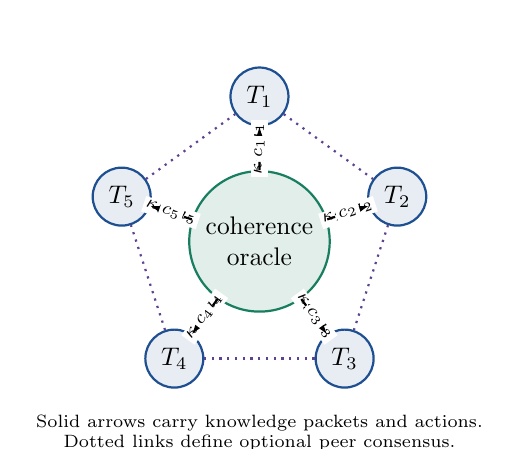
\begin{tikzpicture}[
 scale=0.92,transform shape,
 ag/.style={circle,draw=algblue,fill=algblue!10,thick,minimum size=8mm},
 oracle/.style={circle,draw=alggreen,fill=alggreen!13,thick,minimum size=15mm,align=center},
 arr/.style={-{Latex[length=2mm]},thick},
 msg/.style={font=\scriptsize,fill=white,inner sep=1pt}
]
\node[oracle] (o) at (0,0) {coherence\\oracle};
\foreach \i/\ang in {1/90,2/18,3/-54,4/-126,5/162}{
  \node[ag] (a\i) at (\ang:2.0cm) {$T_{\i}$};
  \draw[arr] (a\i) -- node[msg,sloped] {$\kappa_{\i},a_{\i}$} (o);
  \draw[arr,dashed] (o) -- node[msg,sloped] {$c_{\i}$} (a\i);
}
\draw[algpurple,thick,dotted] (a1) -- (a2);
\draw[algpurple,thick,dotted] (a2) -- (a3);
\draw[algpurple,thick,dotted] (a3) -- (a4);
\draw[algpurple,thick,dotted] (a4) -- (a5);
\draw[algpurple,thick,dotted] (a5) -- (a1);
\node[font=\scriptsize,align=center] at (0,-2.65) {Solid arrows carry knowledge packets and actions.\\Dotted links define optional peer consensus.};
\end{tikzpicture}
\caption{Training-time synchronization. The oracle computes coalition coherence and returns context messages. Peer links can implement finite-round consensus, while the centralized path avoids the impossibility of exact common knowledge over unreliable fully decentralized channels.}
\label{fig:syncgraph}
\end{figure}

\section{Student and Multi-Agent Learning Objectives}
\label{sec:objective}

\subsection{Student Objective}

For minibatch \(B_t\), the student minimizes
\begin{align}
 \cL_S(\theta;\bm a_t)
 =&\ \cL_{\mathrm{sup}}
 +\lambda_L\cL_{\mathrm{logit}}
 +\lambda_F\cL_{\mathrm{feat}}\nonumber\\
 &+\lambda_R\cL_{\mathrm{rel}}
 +\lambda_U\cL_{\mathrm{unc}}
 +\lambda_A\cL_{\mathrm{adapt}},
\label{eq:studenttotal}
\end{align}
where
\begin{equation}
 \cL_{\mathrm{sup}}=-\frac{1}{|B_t|}\sum_{(x,y)\in B_t}\log q_\theta(y\mid x),
\label{eq:supervised}
\end{equation}
\begin{equation}
 \cL_{\mathrm{logit}}
 =\frac{\tau^2}{|B_t|}\sum_{x\in B_t}
 \KL\left(\bar p_t^{(\tau)}(x)\Vert q_\theta^{(\tau)}(x)\right),
\label{eq:logitloss}
\end{equation}
\begin{equation}
 \cL_{\mathrm{feat}}
 =\frac{1}{|B_t|}\sum_{x\in B_t}\sum_{\ell\in\cL}
 \left\|A_S^{(\ell)}h_S^{(\ell)}(x)-\bar k_t^{(\ell)}(x)\right\|_2^2,
\label{eq:featureloss}
\end{equation}
\begin{equation}
 \cL_{\mathrm{rel}}
 =\sum_{\ell\in\cL}\left\|G_S^{(\ell)}-\bar G_t^{(\ell)}\right\|_F^2.
\label{eq:relationloss}
\end{equation}
The uncertainty term can match calibrated confidence or predictive entropy. It is excluded when teacher uncertainty is unreliable.

\subsection{Team Reward}

A reward should measure learning progress rather than the instantaneous ability to imitate teachers. Let \(V_t\) be a held-out validation loss before a student update block and \(V_{t+1}\) the loss after it. The team reward is
\begin{align}
 R_t
 =&\ \underbrace{\frac{V_t-V_{t+1}}{|V_t|+\varepsilon}}_{\text{student progress}}
 +\eta_N\underbrace{\mathrm{Novelty}_t}_{\text{new useful information}}
 -\eta_C\underbrace{\mathrm{CI}_t}_{\text{incoherence}}\nonumber\\
 &-\eta_R\mathrm{Red}_t
 -\eta_X\mathrm{Conf}_t
 -\eta_K\sum_m g_{m,t}
 -\eta_S\|\bm w_t-\bm w_{t-1}\|_2^2.
\label{eq:reward}
\end{align}
Novelty can be estimated from residual packet energy after projection onto the span of active peers,
\begin{equation}
 \mathrm{Novelty}_t
 =\sum_m w_{m,t}\left\|(I-P_{-m,t})\tilde\kappa_{m,t}\right\|_2^2,
\label{eq:novelty}
\end{equation}
where \(P_{-m,t}\) projects onto the packet subspace of the other active teachers. A conditional mutual information estimator can replace this proxy in large-data settings.

\subsection{Difference Rewards}

The global reward can obscure individual contribution. Teacher \(m\) therefore receives
\begin{equation}
 D_{m,t}=R_t(\bm a_t)-R_t(\bm a_{-m,t},a_m^{0}),
\label{eq:differencereward}
\end{equation}
where \(a_m^0\) is a no-teaching action. The leave-one-out student update can be approximated with first-order influence functions rather than an additional full optimization step,
\begin{equation}
 \Delta V_t^{(-m)}\approx
 \Delta V_t-\eta_\theta\left\langle
 \nabla_\theta V_t,
 w_{m,t}\nabla_\theta\cL_{m,t}^{\mathrm{KD}}
 \right\rangle.
\label{eq:influence}
\end{equation}

\subsection{Actor-Critic Objective}

The centralized critic is trained by
\begin{equation}
 \cL_Q(\phi)=\E_t\left[
 \left(Q_\phi(s_t,\bm a_t)-\widehat G_t\right)^2
 \right],
\label{eq:criticloss}
\end{equation}
where \(\widehat G_t\) is a generalized advantage return. Each actor uses a clipped proximal objective,
\begin{align}
 \cJ_m(\omega_m)=\E_t\bigg[\min\big(&r_{m,t}\widehat A_{m,t},\nonumber\\
 &\clip(r_{m,t},1-\epsilon,1+\epsilon)\widehat A_{m,t}\big)\nonumber\\
 &+\eta_H H(\pi_{\omega_m}(\cdot\mid o_{m,t}))\bigg],
\label{eq:mappo}
\end{align}
with probability ratio
\begin{equation}
 r_{m,t}(\omega_m)=
 \frac{\pi_{\omega_m}(a_{m,t}\mid o_{m,t})}
 {\pi_{\omega_m}^{\mathrm{old}}(a_{m,t}\mid o_{m,t})}.
\end{equation}
The advantage can be \(A_{m,t}^{\mathrm{cf}}\), a difference reward return, or a convex combination.

\subsection{Bilevel Formulation}

The complete problem is
\begin{align}
 \max_{\Omega,\phi}\quad &
 J(\Omega)=\E_{\pi_\Omega}\left[\sum_{t=0}^{T}\gamma^tR_t(\theta_t,\bm a_t)\right],
\label{eq:outer}\\
 \text{subject to}\quad &
 \theta_{t+1}=\theta_t-\eta_\theta\nabla_\theta\cL_S(\theta_t;\bm a_t),
\label{eq:inner}\\
 &\E\left[\sum_m g_{m,t}\right]\le B_T,
 \qquad \E[\mathrm{CI}_t]\le \delta_C,
\label{eq:constraints}
\end{align}
where \(\Omega=\{\omega_m\}_{m=1}^{M}\), \(B_T\) is the teacher budget, and \(\delta_C\) is the coherence tolerance. A primal-dual implementation adds learned multipliers for budget and coherence violations.

\section{Formal Theory}
\label{sec:theory}

This section establishes conditional results. The results do not state that every set of teachers is better than every single teacher. Such a claim is false when teachers are duplicated, adversarial, perfectly correlated, or incompatible with the student.

\subsection{Teacher Error Geometry}

Let \(p^*(x)=\Pp(Y=\cdot\mid X=x)\) be the Bayes posterior. For a linear probability barycenter with weights \(\bm w\in\simplex^{M-1}\), define
\begin{equation}
 p_{\bm w}(x)=\sum_{m=1}^{M}w_mp_m(x),
 \qquad e_m(x)=p_m(x)-p^*(x).
\label{eq:errors}
\end{equation}
The teacher error second-moment matrix is
\begin{equation}
 C_{mn}=\E_X\left[\langle e_m(X),e_n(X)\rangle\right].
\label{eq:covmatrix}
\end{equation}
It is symmetric positive semidefinite. Under Brier risk,
\begin{equation}
 \cR_T(\bm w)
 =\E_X\|p_{\bm w}(X)-p^*(X)\|_2^2
 =\bm w^\top C\bm w.
\label{eq:quadraticrisk}
\end{equation}

\begin{theorem}[Multi-Teacher Advantage]
\label{thm:advantage}
Suppose \(C\succ0\), the vector \(C^{-1}\ind\) has strictly positive entries, and the linear barycenter is used. Then the unique minimum-risk interior weight vector is
\begin{equation}
 \bm w^*=\frac{C^{-1}\ind}{\ind^\top C^{-1}\ind},
\label{eq:optimalw}
\end{equation}
with target risk
\begin{equation}
 \cR_T(\bm w^*)=\frac{1}{\ind^\top C^{-1}\ind}.
\label{eq:optimalrisk}
\end{equation}
If
\begin{equation}
 \frac{1}{\ind^\top C^{-1}\ind}+\epsilon_{\mathrm{tr}}^{(M)}
 <\min_m C_{mm}+\underline\epsilon_{\mathrm{tr}}^{(1)},
\label{eq:advcondition}
\end{equation}
where \(\epsilon_{\mathrm{tr}}^{(M)}\) is an upper bound on the student's excess transfer risk for the synchronized coalition target and \(\underline\epsilon_{\mathrm{tr}}^{(1)}\) is a lower bound for admissible single-teacher transfer, then the coordinated multi-teacher student has strictly lower expected Brier risk than every admissible single-teacher student.
\end{theorem}

\begin{proof}
For the equality-constrained interior problem, form
\begin{equation}
 \cJ(\bm w,\lambda)=\bm w^\top C\bm w+\lambda(\ind^\top\bm w-1).
\end{equation}
Stationarity gives \(2C\bm w+\lambda\ind=0\). Since \(C\succ0\),
\begin{equation}
 \bm w=-\frac{\lambda}{2}C^{-1}\ind.
\end{equation}
Imposing \(\ind^\top\bm w=1\) gives \cref{eq:optimalw}. Positivity makes the inequality constraints inactive. Substitution gives \cref{eq:optimalrisk}. The risk of single teacher \(m\) is \(C_{mm}\). Adding the stated transfer-risk bounds to the target risks and applying \cref{eq:advcondition} proves strict advantage.
\end{proof}

\begin{remark}
The condition \(C^{-1}\ind>0\) is sufficient for an interior solution. If it fails, the constrained optimum lies on a face of the simplex and automatically excludes one or more teachers. The same quadratic program still identifies the best coalition.
\end{remark}

\begin{corollary}[Independent unbiased teacher errors]
If teacher errors are uncorrelated with variances \(\sigma_m^2>0\), then
\begin{equation}
 w_m^*=\frac{\sigma_m^{-2}}{\sum_j\sigma_j^{-2}},
 \qquad
 \cR_T(\bm w^*)=\left(\sum_{m=1}^{M}\sigma_m^{-2}\right)^{-1}.
\label{eq:precisionweights}
\end{equation}
For at least two finite-variance teachers, the aggregate target risk is strictly below the risk of the best single teacher.
\end{corollary}

\begin{corollary}[Equicorrelated teachers and diminishing return]
\label{cor:equicorr}
Suppose all teachers have error variance \(\sigma^2\) and pairwise correlation \(\rho\in(-1/(M-1),1)\). Uniform weighting is optimal and
\begin{equation}
 \cR_T(M)=\sigma^2\left(\rho+\frac{1-\rho}{M}\right).
\label{eq:equicorrrisk}
\end{equation}
The gross gain from adding teacher \(M+1\) is
\begin{equation}
 \cR_T(M)-\cR_T(M+1)
 =\frac{\sigma^2(1-\rho)}{M(M+1)}.
\label{eq:marginalgain}
\end{equation}
With per-teacher net cost \(\lambda>0\), the optimal cardinality for this model is the smallest integer \(M^*\) such that
\begin{equation}
 M^*(M^*+1)\ge\frac{\sigma^2(1-\rho)}{\lambda}.
\label{eq:equicorrmstar}
\end{equation}
\end{corollary}

\begin{proof}
The equicorrelation matrix is permutation invariant, so the unique interior optimum is uniform. Expanding the variance of the mean gives \cref{eq:equicorrrisk}. The difference between consecutive risks gives \cref{eq:marginalgain}. Adding teacher \(M+1\) reduces total risk plus cost only when the gross gain exceeds \(\lambda\). The first integer at which that inequality fails is \cref{eq:equicorrmstar}.
\end{proof}

\subsection{Knowledge Coherence}

Let \(K^{(r)}\in\R^{M\times d}\) contain teacher knowledge vectors after synchronization round \(r\). Define the averaging projector
\begin{equation}
 J=\frac{1}{M}\ind\ind^\top,
 \qquad \Pi=I-J,
\end{equation}
and the coherence disagreement
\begin{equation}
 \mathrm{CI}^{(r)}=\frac{1}{M}\|\Pi K^{(r)}\|_F^2.
\label{eq:consensusci}
\end{equation}

\begin{theorem}[Knowledge Coherence]
\label{thm:coherence}
Assume the synchronization matrix \(W\) is doubly stochastic, primitive, and compatible with a connected graph. Let
\begin{equation}
 \rho=\|W-J\|_2<1.
\end{equation}
For exact synchronization \(K^{(r+1)}=WK^{(r)}\),
\begin{equation}
 \mathrm{CI}^{(r)}\le\rho^{2r}\mathrm{CI}^{(0)},
\label{eq:coherencecontraction}
\end{equation}
and every teacher message converges to the common average \(JK^{(0)}\). If bounded perturbations satisfy
\begin{equation}
 \|\Pi E^{(r)}\|_F\le\varepsilon_E,
\end{equation}
then
\begin{equation}
 \sqrt{\mathrm{CI}^{(r)}}
 \le\rho^r\sqrt{\mathrm{CI}^{(0)}}
 +\frac{\varepsilon_E}{\sqrt{M}(1-\rho)}.
\label{eq:coherencefloor}
\end{equation}
Consequently, bounded communication perturbations create a nonzero coherence floor.
\end{theorem}

\begin{proof}
Because \(W\) is doubly stochastic, \(WJ=JW=J\), and therefore
\begin{equation}
 \Pi K^{(r+1)}=(W-J)\Pi K^{(r)}
\end{equation}
for exact synchronization. Submultiplicativity gives
\begin{equation}
 \|\Pi K^{(r)}\|_F\le\rho^r\|\Pi K^{(0)}\|_F,
\end{equation}
which proves \cref{eq:coherencecontraction}. With perturbation,
\begin{equation}
 \|\Pi K^{(r+1)}\|_F
 \le\rho\|\Pi K^{(r)}\|_F+\varepsilon_E.
\end{equation}
Unrolling the scalar recurrence yields
\begin{equation}
 \|\Pi K^{(r)}\|_F
 \le\rho^r\|\Pi K^{(0)}\|_F
 +\varepsilon_E\sum_{j=0}^{r-1}\rho^j.
\end{equation}
The geometric sum is bounded by \((1-\rho)^{-1}\). Division by \(\sqrt{M}\) proves \cref{eq:coherencefloor}.
\end{proof}

\begin{corollary}[Target stability]
If the synchronized target map \(F(K)\) is \(L_F\)-Lipschitz in Frobenius norm, then
\begin{equation}
 \|F(K^{(r)})-F(JK^{(0)})\|_2
 \le L_F\left(\rho^r\|\Pi K^{(0)}\|_F+\frac{\varepsilon_E}{1-\rho}\right).
\label{eq:targetstability}
\end{equation}
Thus, the student target is stable up to the same spectral and communication floor.
\end{corollary}

\begin{remark}
The theorem does not contradict common-knowledge impossibility results. It assumes a connected mixing process and bounded perturbations during centralized training. Exact coherence is not promised when messages can be lost forever, delays are unbounded, or the target changes faster than the synchronization process contracts.
\end{remark}

\subsection{Teacher Saturation}

Let \(\cS_M\) be a nested sequence of selected teacher sets and let \(K_{\cS_M}\) denote their aggregate knowledge message. Define gross teacher information
\begin{equation}
 G_M=I(Y;K_{\cS_M}).
\label{eq:grossinfo}
\end{equation}
For the next selected teacher \(j_{M+1}\), the chain rule gives
\begin{equation}
 g_{M+1}=G_{M+1}-G_M
 =I(Y;K_{j_{M+1}}\mid K_{\cS_M}).
\label{eq:conditionalgain}
\end{equation}
Let \(Z_M\) be the student representation formed from the teacher message through a bounded distillation channel, with
\begin{equation}
 I(Z_M;K_{\cS_M})\le B_S.
\label{eq:capacity}
\end{equation}

\begin{theorem}[Teacher Saturation]
\label{thm:saturation}
Assume the Markov chain \(Y\to K_{\cS_M}\to Z_M\), the capacity bound in \cref{eq:capacity}, nonincreasing gains \(g_{M+1}\), and a nondecreasing incremental coordination cost \(d_{M+1}=C_{M+1}-C_M\ge d_0>0\). Then:

\begin{enumerate}
    \item The student-usable teacher information satisfies
    \begin{equation}
    I(Y;Z_M)\le \min\{G_M,B_S\}.
    \label{eq:usableinfo}
    \end{equation}
    \item For net value
    \begin{equation}
    U_M=\min\{G_M,B_S\}-C_M,
    \label{eq:netutility}
    \end{equation}
    there exists a finite optimal cardinality \(M^*\).
    \item A sufficient stopping condition is
    \begin{equation}
    \min\left\{g_{M+1},[B_S-G_M]_+\right\}\le d_{M+1}.
    \label{eq:stoprule}
    \end{equation}
    Once \cref{eq:stoprule} holds, no later teacher in the nested diminishing-return sequence can increase net value.
\end{enumerate}
\end{theorem}

\begin{proof}
The data processing inequality gives \(I(Y;Z_M)\le I(Y;K_{\cS_M})=G_M\). Also, \(I(Y;Z_M)\le I(K_{\cS_M};Z_M)\le B_S\), which proves \cref{eq:usableinfo}. The incremental net value is
\begin{equation}
 U_{M+1}-U_M
 =\min\{g_{M+1},[B_S-G_M]_+\}-d_{M+1}.
\label{eq:netincrement}
\end{equation}
The first term is nonincreasing because the conditional gains are nonincreasing and the remaining capacity is nonincreasing. The second term is nondecreasing and bounded below by a positive constant. Therefore, the increments eventually become non-positive and remain non-positive. This proves finite saturation and the stopping rule.
\end{proof}

\begin{corollary}[Rank-limited student]
If all synchronized teacher features lie in a subspace of rank \(r_T\), while the student adapter can represent at most rank \(r_S\), then useful independent feature directions cannot exceed \(\min(r_T,r_S)\). Once the selected teacher packet span reaches this rank and residual conditional information is zero, additional teachers can only reduce risk through repeated noisy measurements, not through new representational directions.
\end{corollary}

\begin{proposition}[More teachers can be worse]
There exist teacher pools for which equal-weight multi-teacher distillation has larger target risk than the best single teacher.
\end{proposition}

\begin{proof}
Let teacher one be perfect, \(e_1=0\), and teacher two have nonzero error \(e_2\). The best single-teacher risk is zero. Equal averaging produces error \(e_2/2\) and positive risk \(\E\|e_2\|_2^2/4\). This counterexample shows why teacher selection and weighting are necessary.
\end{proof}

\begin{figure}[t]
\centering
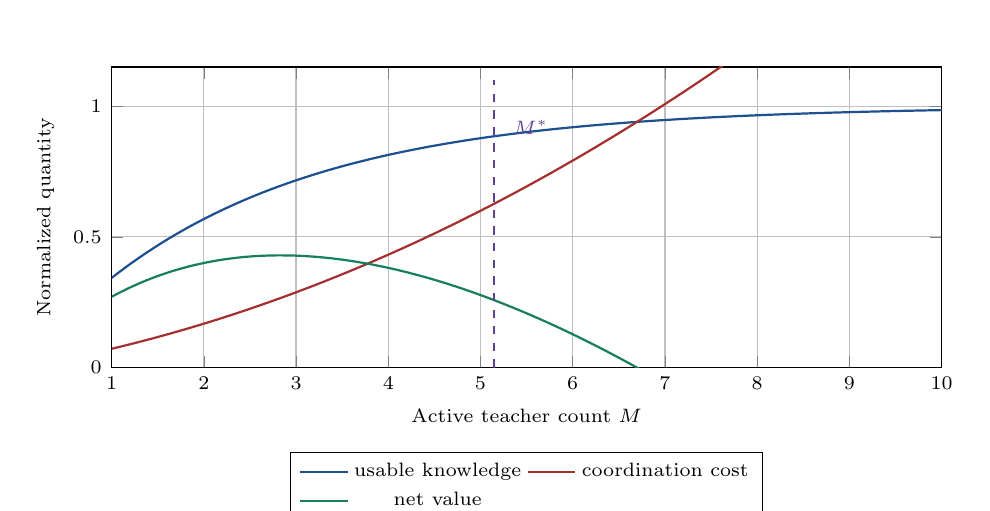
\begin{tikzpicture}
\begin{axis}[
 width=\columnwidth,
 height=5.4cm,
 xlabel={Active teacher count $M$},
 ylabel={Normalized quantity},
 xmin=1,xmax=10,
 ymin=0,ymax=1.15,
 grid=both,
 legend style={font=\scriptsize,at={(0.5,-0.28)},anchor=north,legend columns=2},
 tick label style={font=\scriptsize},
 label style={font=\scriptsize}
]
\addplot[algblue,thick,domain=1:10,samples=100]{1-exp(-0.42*x)};
\addlegendentry{usable knowledge}
\addplot[algred,thick,domain=1:10,samples=100]{0.06*x+0.012*x^2};
\addlegendentry{coordination cost}
\addplot[alggreen,thick,domain=1:10,samples=100]{1-exp(-0.42*x)-0.06*x-0.012*x^2};
\addlegendentry{net value}
\addplot[dashed,algpurple,thick] coordinates {(5.15,0) (5.15,1.1)};
\node[font=\scriptsize,algpurple,anchor=west] at (axis cs:5.25,0.92) {$M^*$};
\end{axis}
\end{tikzpicture}
\caption{Conceptual saturation curve. Teacher information increases with diminishing returns, while communication, conflict, and compute costs increase. The optimal cardinality occurs near the maximum of net value. This is a theoretical illustration, not an empirical result.}
\label{fig:saturation}
\end{figure}

\section{Algorithms}
\label{sec:algorithms}

\begin{algorithm}[t]
\caption{CoMTKD-MARL Training}
\label{alg:training}
\begin{algorithmic}[1]
\Require Teacher pool \(\cT\), student \(S_\theta\), actors \(\{\pi_{\omega_m}\}\), critic \(Q_\phi\), training and validation data
\State Calibrate teachers and initialize adapters
\State Warm-start student with supervised loss or equal-weight KD
\State Warm-start critic from random teacher coalitions
\For{decision epoch \(t=0,\ldots,T-1\)}
    \State Sample training minibatch \(B_t\) and validation minibatch \(B_t^v\)
    \ForAll{teachers \(m\) in parallel}
        \State Compute packet \(\kappa_{m,t}\) and observation \(o_{m,t}\)
        \State Sample action \(a_{m,t}\sim\pi_{\omega_m}(\cdot\mid o_{m,t})\)
    \EndFor
    \State Normalize gates and weights using \cref{eq:weights}
    \State Synchronize active packets using Algorithm \ref{alg:sync}
    \State Compute \(\cL_S\) using \cref{eq:studenttotal}
    \State Update student for \(K_S\) gradient steps
    \State Evaluate progress and compute team reward \cref{eq:reward}
    \State Estimate counterfactual advantages or difference rewards
    \State Store \((s_t,\bm o_t,\bm a_t,R_t,s_{t+1})\)
    \If{actor-critic update interval reached}
        \State Update critic with \cref{eq:criticloss}
        \State Update actors with clipped objective \cref{eq:mappo}
        \State Update budget and coherence multipliers
    \EndIf
    \State Update cardinality controller using Algorithm \ref{alg:cardinality}
\EndFor
\State Select best validation checkpoint and discard all teacher-side modules
\Ensure Deployed student \(S_{\theta^*}\)
\end{algorithmic}
\end{algorithm}

\begin{algorithm}[t]
\caption{Knowledge Synchronization}
\label{alg:sync}
\begin{algorithmic}[1]
\Require Active packets \(\{\kappa_m\}_{m\in\cS}\), weights \(\bm w\), graph \(\cG\), rounds \(R_s\)
\State Project logits, features, relations, and uncertainty to common spaces
\State Stack packet embeddings as \(K^{(0)}\)
\For{round \(r=0,\ldots,R_s-1\)}
    \State Construct or update doubly stochastic mixing matrix \(W^{(r)}\)
    \State Exchange compressed packet summaries
    \State \(K^{(r+1)}\gets W^{(r)}K^{(r)}+E^{(r)}\)
    \If{coherence index is below tolerance}
        \State \textbf{break}
    \EndIf
\EndFor
\State Compute logit barycenter \(\bar p\), feature target \(\bar k\), relation target \(\bar G\)
\State Compute \(\mathrm{CI}\), redundancy, conflict, and novelty
\Ensure Synchronized target and indicators
\end{algorithmic}
\end{algorithm}

\begin{algorithm}[t]
\caption{Adaptive Teacher Cardinality}
\label{alg:cardinality}
\begin{algorithmic}[1]
\Require Marginal estimates \(\widehat\Delta_m\), confidence radii \(b_m\), incremental costs \(d_m\), current set \(\cS_t\)
\ForAll{teachers \(m\)}
    \State \(\mathrm{LCB}_m\gets\widehat\Delta_m-b_m-d_m\)
    \State \(\mathrm{UCB}_m\gets\widehat\Delta_m+b_m-d_m\)
\EndFor
\State Remove active teacher \(m\) when \(\mathrm{UCB}_m\le0\) for \(H\) consecutive checks
\State Add inactive teacher \(j\) when \(\mathrm{LCB}_j>0\) and budget permits
\State Enforce minimum and maximum coalition size
\State If all inactive upper bounds are non-positive, declare saturation
\Ensure Updated active set \(\cS_{t+1}\) and estimated \(M_t^*\)
\end{algorithmic}
\end{algorithm}

\section{Complexity and Scaling}
\label{sec:complexity}

Let \(B\) be minibatch size, \(M_a\) the active teacher count, \(C\) the class count, \(d\) the synchronized feature dimension, \(|E|\) the synchronization-graph edge count, and \(R_s\) the number of consensus rounds. Teacher forward passes cost the sum of active teacher inference costs. The additional aggregation cost is
\begin{equation}
 O\left(BM_a(C+d)+R_sB|E|d\right).
\label{eq:aggregationcomplexity}
\end{equation}
Computing all pairwise redundancy and conflict scores is \(O(BM_a^2d)\), but a sparse neighbor graph or low-rank sketch reduces this to \(O(B|E|d)\). A centralized critic that concatenates every agent state scales at least linearly in \(M_a\), while attention pooling or a graph critic supports variable teacher counts.

Memory overhead includes active teacher activations, packet embeddings, actor trajectories, and influence estimates. Feature packets should be detached from teacher graphs when teachers are frozen. Gradient conflict can be computed from projected gradients or last-layer gradients to avoid storing complete per-teacher gradients.

Inference complexity is unchanged from the student baseline. Teachers, actors, critic, oracle, and cardinality controller are training-only components.

\section{Experimental Evaluation Protocol}
\label{sec:experiments}

This manuscript does not report fabricated empirical values. The following protocol is designed to test, and potentially falsify, the theoretical claims.

\subsection{Tasks and Teacher Pools}

The core vision evaluation should include CIFAR-100 and ImageNet-1K classification, COCO object detection, and ADE20K or Cityscapes semantic segmentation. Teacher pools should vary along controlled axes:

\begin{itemize}
    \item architecture diversity, for example convolutional networks, vision transformers, and hybrid networks;
    \item accuracy and calibration diversity;
    \item training-data diversity, including class imbalance and domain shift;
    \item error correlation, created through shared or independent initializations and augmentations;
    \item capacity gap relative to the student;
    \item adversarial or corrupted teachers with label noise, stale checkpoints, or targeted class errors.
\end{itemize}

An optional language-model study can use multiple reasoning or domain-specialist teachers to distill a compact decoder model. The same theory applies, but token-level sequence dependence requires autoregressive variants of the knowledge packet and reward.

\subsection{Baselines}

Required baselines are supervised student training, best single teacher, strongest teacher, equal-weight multi-teacher KD, entropy or confidence weighting, gradient-space adaptive ensemble KD, MTKD-RL, and \CoMTKD variants without synchronization, without difference rewards, and without cardinality control. MARL ablations should compare independent PPO, MAPPO, MADDPG, and a monotonic value-factorization critic when actions are discretized.

\subsection{Teacher Cardinality Sweep}

For each teacher pool, evaluate nested and non-nested coalitions for \(M=1,\ldots,M_{\max}\). Report student accuracy or task metric, calibration, negative log-likelihood, Brier score, training cost, active teacher count, coherence, redundancy, conflict, and marginal contribution. The cardinality controller is successful only if its selected \(M^*\) is close to the validation-optimal count and remains stable across seeds.

\subsection{Theorem-Oriented Measurements}

Estimate the error second-moment matrix \(C\) on held-out data and solve the simplex quadratic program. Compare predicted barycentric risk with measured aggregate risk. For \cref{thm:advantage}, report the covariance condition, target-risk gap, transfer excess, and whether the sufficient condition holds before examining student performance.

For \cref{thm:coherence}, measure \(\mathrm{CI}^{(r)}\) across synchronization rounds and estimate the contraction factor from the second singular value of the mixing matrix. Inject packet loss, quantization, bounded delay, and stale packets. The theorem is corroborated if disagreement contracts geometrically in the reliable regime and approaches a perturbation-dependent floor in the noisy regime.

For \cref{thm:saturation}, estimate conditional novelty with residual features and, when feasible, neural mutual information estimators. Compare the empirical next-teacher gain with incremental cost. The theorem is challenged if gains systematically increase after the stopping condition under the stated nested diminishing-return assumptions.

\subsection{Metrics}

\begin{table}[t]
\caption{Core evaluation metrics}
\label{tab:metrics}
\centering
\footnotesize
\begin{tabularx}{\columnwidth}{@{}p{0.28\columnwidth}X@{}}
\toprule
Category & Metrics \\
\midrule
Student quality & Accuracy, F1, mAP, mIoU, NLL, Brier score, ECE \\
Teacher value & Leave-one-out gain, conditional novelty, gradient alignment \\
Coordination & Logit CI, feature CI, conflict rate, weight variation \\
Saturation & Selected count, oracle-optimal count, regret, stopping delay \\
Efficiency & GPU hours, peak memory, teacher forward passes, wall time \\
Robustness & Packet-loss sensitivity, stale-teacher sensitivity, adversarial-teacher tolerance \\
\bottomrule
\end{tabularx}
\end{table}

\subsection{Statistical Design}

Use at least five independent seeds for large-scale experiments and ten seeds for smaller benchmarks. Report means, standard deviations, paired confidence intervals, and effect sizes. Use paired permutation tests or hierarchical bootstrap intervals across seeds and classes. Correct families of multiple comparisons with Holm's method. Hyperparameters must be selected on validation data without using test performance. Publish teacher checkpoints, coalition definitions, code, random seeds, hardware details, and the exact calculation of every coherence and cardinality metric.

\subsection{Falsification Criteria}

\begin{enumerate}
    \item The Multi-Teacher Advantage claim is not supported when the covariance-based sufficient condition holds with a meaningful margin but the synchronized student is consistently worse than all single-teacher students after optimization error is controlled.
    \item The Knowledge Coherence claim is not supported when a fixed connected mixing graph fails to contract disagreement at the predicted spectral rate in the absence of perturbation.
    \item The Teacher Saturation claim is not supported when conditional gains and remaining student capacity are both below incremental cost, yet later teachers consistently improve net validation value under the same nested sequence.
    \item The architecture claim is weakened if independent teacher actors match the full method on conflict-heavy and communication-stressed pools.
\end{enumerate}

\section{Discussion}
\label{sec:discussion}

\subsection{Why Multi-Agent Reinforcement Learning Is Needed}

A single weighting network can choose teacher weights, and for small homogeneous pools it may be sufficient. The multi-agent formulation becomes useful when teachers have distinct observations, costs, modalities, or action spaces. It also makes marginal credit explicit. Each teacher actor can learn a local policy, while the critic reasons about coalition interactions. The formulation supports teachers joining or leaving, sparse communication, and teacher-specific constraints.

\subsection{Why Synchronization Is Separate from Weighting}

Weighting answers how much each teacher contributes. Synchronization answers whether their messages refer to comparable representations and whether the joint target is internally stable. A low weight does not repair an unaligned feature space. Conversely, perfect feature alignment does not determine whether a teacher adds novel information. The architecture separates these roles and exposes both to the reward.

\subsection{Interpretation of Optimal Cardinality}

The optimal count is not a universal constant. It depends on error correlation, student capacity, task complexity, sample region, training phase, and coordination cost. Early training may benefit from broad, smooth supervision, while late training may prefer a smaller set of precise specialists. The learned cardinality can therefore be sample-wise, epoch-wise, or globally constrained.

\subsection{Failure Modes}

The main failure modes are reward leakage from a reused validation set, actor collapse onto one teacher, collusion among correlated teachers, unstable teacher switching, inaccurate mutual information estimation, and critic overfitting. Mitigations include a rotating reward-validation buffer, entropy and diversity regularization, influence-based audits, hysteresis, confidence bounds, and a held-out final selection set.

\subsection{Limitations}

The Multi-Teacher Advantage Theorem uses a linear probability barycenter and Brier geometry. Kullback-Leibler loss has a local quadratic approximation, but global equivalence requires probabilities bounded away from zero. The coherence theorem describes the synchronization operator, not convergence of the complete nonconvex student and actor optimization. The saturation theorem requires diminishing conditional novelty along the selected sequence and a bounded student information channel. Mutual information is difficult to estimate in high dimensions. Teacher actors increase training cost, and the method is most justified when the teacher pool is expensive enough that poor selection would also be expensive.

The framework does not guarantee safety against deliberately adversarial teachers. Robust aggregation, trust scores, signed interaction graphs, and Byzantine-resistant synchronization are necessary extensions in that setting.

\subsection{Broader Impact}

Coordinated distillation can reduce inference energy and make strong models deployable on constrained devices. It can also reproduce hidden teacher biases and obscure provenance when many teachers contribute. Implementations should record teacher identities, weights, selected channels, conflict indicators, and data licenses. Sensitive applications should audit whether minority classes are repeatedly assigned to weak or biased teachers.

\section{Conclusion}

This paper developed \CoMTKD, a coherent multi-teacher distillation framework based on cooperative multi-agent reinforcement learning. The architecture distinguishes teacher relevance, knowledge synchronization, cooperative credit, and cardinality control. Its student objective combines supervised, logit, feature, and relational learning, while the teacher agents optimize delayed validation progress under coherence, redundancy, conflict, stability, and cost penalties.

The formal analysis establishes three conclusions under explicit assumptions. A diverse teacher coalition can outperform every single teacher when its error covariance supports beneficial averaging and the student can absorb the synchronized target. Connected synchronization contracts disagreement geometrically, while bounded communication noise produces a measurable coherence floor. Teacher value eventually saturates because conditional novelty decreases, student information capacity is finite, and coordination cost increases. These results replace the informal claim that more teachers are always better with a testable statement about when multiple teachers help, how their knowledge should be coordinated, and when the teaching coalition should stop growing.

\appendix

\section{Notation Summary}

\begin{table*}[t]
\caption{Principal notation}
\label{tab:notation}
\centering
\small
\begin{tabularx}{0.96\textwidth}{@{}p{0.16\textwidth}X p{0.16\textwidth}X@{}}
\toprule
Symbol & Meaning & Symbol & Meaning \\
\midrule
\(M\) & Number of available teachers & \(M_t\) & Number of active teachers at epoch \(t\) \\
\(T_m\) & Teacher model \(m\) & \(S_\theta\) & Student model with parameters \(\theta\) \\
\(p_m\) & Teacher predictive distribution & \(q_\theta\) & Student predictive distribution \\
\(\kappa_m\) & Teacher knowledge packet & \(w_m\) & Normalized teacher weight \\
\(g_m\) & Teacher participation gate & \(\bm\beta_m\) & Teaching-channel allocation \\
\(K^{(r)}\) & Packet matrix after synchronization round \(r\) & \(W\) & Consensus mixing matrix \\
\(\mathrm{CI}\) & Coherence disagreement index & \(C\) & Teacher error second-moment matrix \\
\(B_S\) & Student information capacity & \(G_M\) & Gross information in selected teacher set \\
\(g_{M+1}\) & Conditional information gain of next teacher & \(M^*\) & Optimal teacher cardinality \\
\bottomrule
\end{tabularx}
\end{table*}

\section{Additional Proof Details}

\subsection{Kullback-Leibler Local Corollary}

Suppose all teacher, aggregate, and Bayes probabilities lie in
\begin{equation}
 \simplex_\delta^{C-1}=\{p\in\simplex^{C-1}:p_c\ge\delta\text{ for all }c\},
\end{equation}
for \(\delta>0\). On this compact interior, the Hessian of negative entropy is bounded. Therefore, constants \(0<c_\delta\le C_\delta<\infty\) exist such that
\begin{equation}
 c_\delta\|p-q\|_2^2
 \le\KL(p\Vert q)
 \le C_\delta\|p-q\|_2^2.
\label{eq:klequiv}
\end{equation}
Consequently, a strict Brier-risk advantage with margin larger than the equivalence and transfer-error slack implies a Kullback-Leibler advantage. This corollary does not cover teachers that assign zero probability to plausible classes.

\subsection{Weighted Consensus}

When teacher weights are fixed and nonuniform, let \(\bm w\) be the stationary distribution of a primitive row-stochastic matrix \(W\), so \(\bm w^\top W=\bm w^\top\). Define \(J_w=\ind\bm w^\top\). If
\begin{equation}
 \rho_w=\|W-J_w\|_{\bm w}<1
\end{equation}
under the weighted Euclidean norm, then
\begin{equation}
 \|K^{(r)}-J_wK^{(0)}\|_{\bm w}
 \le\rho_w^r\|K^{(0)}-J_wK^{(0)}\|_{\bm w}.
\end{equation}
The common limit is the actor-weighted knowledge barycenter.

\subsection{Saturation with Explicit Coherence Cost}

Let
\begin{equation}
 C_M=\lambda_KM+\lambda_C\delta_M+\lambda_R r_M,
\end{equation}
where \(\delta_M\) is expected incoherence and \(r_M\) is expected redundancy. The incremental cost is
\begin{equation}
 d_{M+1}=\lambda_K+\lambda_C(\delta_{M+1}-\delta_M)
 +\lambda_R(r_{M+1}-r_M).
\end{equation}
The stopping condition becomes
\begin{equation}
 \min\{g_{M+1},[B_S-G_M]_+\}
 \le\lambda_K+\lambda_C\Delta\delta_{M+1}+\lambda_R\Delta r_{M+1}.
\label{eq:explicitstop}
\end{equation}
This equation directly links the theoretical cardinality threshold to measurable training indicators.

\section{Recommended Implementation Configuration}

A practical first implementation can use four to eight teachers, MAPPO actors with shared parameters plus teacher identifiers, an attention-based centralized critic, three teaching channels, and one synchronization round through a centralized barycenter. Start with a gate cost that targets two to four active teachers, then anneal the cost only after the student warm start. Update teacher actors less frequently than the student, for example once after several student minibatches, because the validation reward is otherwise dominated by noise.

The critic state should include current student loss, a moving validation loss, the full weight vector, active count, teacher confidence, teacher-student Kullback-Leibler gaps, pairwise coherence summaries, and recent difference rewards. Full feature tensors should not be passed to the critic. Pool them into stable statistics or low-rank sketches.

\begin{table}[h]
\caption{Suggested starting hyperparameters}
\label{tab:hparams}
\centering
\footnotesize
\begin{tabular}{@{}ll@{}}
\toprule
Quantity & Starting range \\
\midrule
Student learning rate & \(10^{-4}\) to \(3\times10^{-3}\) \\
Actor learning rate & \(10^{-5}\) to \(3\times10^{-4}\) \\
Critic learning rate & \(3\times10^{-5}\) to \(10^{-3}\) \\
PPO clip & \(0.1\) to \(0.2\) \\
Discount factor & \(0.95\) to \(0.995\) \\
GAE parameter & \(0.90\) to \(0.97\) \\
Teacher temperature & \(1\) to \(8\) \\
Consensus rounds & \(1\) to \(5\) \\
Cardinality dwell time & \(5\) to \(20\) checks \\
Coherence penalty & selected by validation constraint \\
\bottomrule
\end{tabular}
\end{table}

\section{Reproducibility Checklist}

A complete release should include the following.

\begin{itemize}
    \item Exact teacher checkpoints, training data, and calibration procedure.
    \item Student initialization and all adapter architectures.
    \item Observation normalization, actor action transforms, and gate thresholds.
    \item Reward computation, validation-buffer rotation, and influence approximation.
    \item Synchronization graph, mixing matrices, packet compression, and perturbation model.
    \item Random seeds, number of runs, hardware, software versions, and wall-clock cost.
    \item Raw per-epoch teacher weights, active sets, coherence metrics, and marginal utilities.
    \item Scripts that reproduce theorem-oriented covariance, spectral, and saturation analyses.
\end{itemize}

\balance
\begin{thebibliography}{99}

\bibitem{hinton2015}
G. Hinton, O. Vinyals, and J. Dean, ``Distilling the knowledge in a neural network,'' in \emph{NIPS Deep Learning and Representation Learning Workshop}, 2015, arXiv:1503.02531.

\bibitem{romero2015}
A. Romero, N. Ballas, S. E. Kahou, A. Chassang, C. Gatta, and Y. Bengio, ``FitNets: Hints for thin deep nets,'' in \emph{International Conference on Learning Representations}, 2015.

\bibitem{cho2019}
J. H. Cho and B. Hariharan, ``On the efficacy of knowledge distillation,'' in \emph{IEEE International Conference on Computer Vision}, pp. 4794--4802, 2019.

\bibitem{stanton2021}
S. Stanton, P. Izmailov, P. Kirichenko, A. A. Alemi, and A. G. Wilson, ``Does knowledge distillation really work?'' in \emph{Advances in Neural Information Processing Systems}, vol. 34, 2021.

\bibitem{zhu2022}
Y. Zhu, N. Liu, Z. Xu, X. Liu, W. Meng, L. Wang, Z. Ou, and J. Tang, ``Teach less, learn more: On the undistillable classes in knowledge distillation,'' in \emph{Advances in Neural Information Processing Systems}, vol. 35, 2022.

\bibitem{park2021}
D. Y. Park, M.-H. Cha, C. Jeong, D. Kim, and B. Han, ``Learning student-friendly teacher networks for knowledge distillation,'' in \emph{Advances in Neural Information Processing Systems}, vol. 34, 2021.

\bibitem{du2020}
S. Du, S. You, X. Li, J. Wu, F. Wang, C. Qian, and C. Zhang, ``Agree to disagree: Adaptive ensemble knowledge distillation in gradient space,'' in \emph{Advances in Neural Information Processing Systems}, vol. 33, 2020.

\bibitem{yang2025}
C. Yang, X. Yu, H. Yang, Z. An, C. Yu, L. Huang, and Y. Xu, ``Multi-teacher knowledge distillation with reinforcement learning for visual recognition,'' arXiv:2502.18510, 2025.

\bibitem{panigrahi2026}
A. Panigrahi, B. Liu, S. Malladi, S. M. Kakade, and S. Goel, ``In good GRACEs: Principled teacher selection for knowledge distillation,'' in \emph{International Conference on Learning Representations}, 2026.

\bibitem{lowe2017}
R. Lowe, Y. Wu, A. Tamar, J. Harb, P. Abbeel, and I. Mordatch, ``Multi-agent actor-critic for mixed cooperative-competitive environments,'' in \emph{Advances in Neural Information Processing Systems}, vol. 30, 2017.

\bibitem{foerster2018}
J. Foerster, G. Farquhar, T. Afouras, N. Nardelli, and S. Whiteson, ``Counterfactual multi-agent policy gradients,'' in \emph{Proceedings of the AAAI Conference on Artificial Intelligence}, vol. 32, no. 1, pp. 2974--2982, 2018.

\bibitem{rashid2018}
T. Rashid, M. Samvelyan, C. Schroeder de Witt, G. Farquhar, J. Foerster, and S. Whiteson, ``QMIX: Monotonic value function factorisation for deep multi-agent reinforcement learning,'' in \emph{Proceedings of the 35th International Conference on Machine Learning}, vol. 80, pp. 4295--4304, 2018.

\bibitem{yu2022}
C. Yu, A. Velu, E. Vinitsky, J. Gao, Y. Wang, A. Bayen, and Y. Wu, ``The surprising effectiveness of PPO in cooperative multi-agent games,'' in \emph{Advances in Neural Information Processing Systems}, vol. 35, 2022.

\bibitem{schulman2017}
J. Schulman, F. Wolski, P. Dhariwal, A. Radford, and O. Klimov, ``Proximal policy optimization algorithms,'' arXiv:1707.06347, 2017.

\bibitem{halpern1990}
J. Y. Halpern and Y. Moses, ``Knowledge and common knowledge in a distributed environment,'' \emph{Journal of the ACM}, vol. 37, no. 3, pp. 549--587, 1990.

\bibitem{olfati2007}
R. Olfati-Saber, J. A. Fax, and R. M. Murray, ``Consensus and cooperation in networked multi-agent systems,'' \emph{Proceedings of the IEEE}, vol. 95, no. 1, pp. 215--233, 2007.

\bibitem{boyd2006}
S. Boyd, A. Ghosh, B. Prabhakar, and D. Shah, ``Randomized gossip algorithms,'' \emph{IEEE Transactions on Information Theory}, vol. 52, no. 6, pp. 2508--2530, 2006.

\bibitem{chiurunge2026}
P. Chiurunge, ``A formal theory of failure in decentralized and LLM-based multi-agent systems: Linking epistemic divergence, non-stationary learning, bounded communication, and memory decay into a unified failure taxonomy with measurable early-warning indicators,'' unpublished manuscript, Deep Analytics, Harare, Zimbabwe, 2026.

\bibitem{nemhauser1978}
G. L. Nemhauser, L. A. Wolsey, and M. L. Fisher, ``An analysis of approximations for maximizing submodular set functions,'' \emph{Mathematical Programming}, vol. 14, pp. 265--294, 1978.

\bibitem{krause2014}
A. Krause and D. Golovin, ``Submodular function maximization,'' in \emph{Tractability: Practical Approaches to Hard Problems}, L. Bordeaux, Y. Hamadi, and P. Kohli, Eds. Cambridge, United Kingdom: Cambridge University Press, pp. 71--104, 2014.

\bibitem{tishby1999}
N. Tishby, F. C. Pereira, and W. Bialek, ``The information bottleneck method,'' in \emph{Proceedings of the 37th Annual Allerton Conference on Communication, Control, and Computing}, pp. 368--377, 1999.

\bibitem{cover2006}
T. M. Cover and J. A. Thomas, \emph{Elements of Information Theory}, 2nd ed. Hoboken, NJ, USA: Wiley, 2006.

\bibitem{jang2017}
E. Jang, S. Gu, and B. Poole, ``Categorical reparameterization with Gumbel-Softmax,'' in \emph{International Conference on Learning Representations}, 2017.

\bibitem{li2023}
L. Li, P. Dong, A. Li, Z. Wei, and Y. Yang, ``KD-Zero: Evolving knowledge distiller for any teacher-student pairs,'' in \emph{Advances in Neural Information Processing Systems}, vol. 36, 2023.

\bibitem{ojha2023}
U. Ojha, Y. Li, A. S. Rajan, Y. Liang, and Y. J. Lee, ``What knowledge gets distilled in knowledge distillation?'' in \emph{Advances in Neural Information Processing Systems}, vol. 36, 2023.

\bibitem{huang2023}
T. Huang, Y. Zhang, M. Zheng, S. You, F. Wang, C. Qian, and C. Xu, ``Knowledge diffusion for distillation,'' in \emph{Advances in Neural Information Processing Systems}, vol. 36, 2023.

\bibitem{liu2024}
J. Liu, C. Zhang, J. Guo, Y. Zhang, H. Que, K. Deng, Z. Bai, J. Liu, G. Zhang, J. Wang, Y. Wu, C. Liu, J. Wang, L. Qu, W. Su, and B. Zheng, ``DDK: Distilling domain knowledge for efficient large language models,'' in \emph{Advances in Neural Information Processing Systems}, vol. 37, 2024.

\end{thebibliography}

\end{document}
